\chapter{Problemanalyse}
\textit{I dette kapitel analyses problemstillinger, som opstår i forbindelse med lægemiddelskift og hvordan disse problemstillinger kan forebygges. Problemstillingerne vil sammenfattes i en opsummering og afsluttes med en problemformulering, der fremadrettet danner grundlaget for rapporten.}

\section{Lægemiddelskift}
%\textit{Hvad er et lægemiddelskift, hvorfor sker det og hvad medfører det?} \\
Udgifterne til sygehusmedicin er stigende i flere europæiske lande, hvorfor flere lægemidler substitueres, med henblik på at opnå besparelser på medicin~\citep{Ess2003,Johnston2011}. Ved substitution udskiftes et lægemiddel til et andet lægemiddel og kategoriseres som generisk eller analog~\citep{DanskSelskabforPatientsikkerhed2009, Kairi2017}. Generisk substitution er substitution af lægemidler, der er  generisk ækvivalent med det forskrevne lægemiddel, herunder samme aktive stof, identiske styrke, koncentration og administrationsvej~\citep{DanskSelskabforPatientsikkerhed2009, Kairi2017}. Dette kan give anledning til at lægemidlets navn skifter eller varemærket ændres~\citep{Kairi2017}. Analog substitution er alle lægemidler, som ikke er generiske~\citep{Kairi2017}. Disse afviger i sammensætningen, men anses for at have lignende bivirkninger og terapeutiske egenskaber~\citep{DanskSelskabforPatientsikkerhed2009, Kairi2017}.


\section{Patientsikkerhedsmæssige konsekvenser} \label{sec:ProblemLaeg} %Problemer ved lægemiddelskift i klinikken} \label{sec:ProblemLaeg}
%\textit{Hvilke patientsikkerhedsmæssige konsekvenser opstår og hvorfor opstår disse?} \\
Substitution kan lede til patientsikkerhedsmæssige konsekvenser~\citep{DanskSelskabforPatientsikkerhed2009}. En af årsagerne er at producenter af lægemidler kan anvende forskellige hjælpestoffer, som på trods af kliniske forsøg, kan påvirke patienter forskelligt i forhold til optagelse og interaktion med andre lægemidler~\citep{Kairi2017}. Lægemidlet, som erstattes, kan have en anderledes form, størrelse eller farve end det forskrevne lægemiddel, hvormed patienten kan undlade at tage medicinen på grund af mistanke om fejl i ordination~\citep{Kairi2017}. Analog substitution kan alene medvirke til at lægemidlet inden for samme farmakologiske klasse afviger i forhold til biologiske virkning, men dette er endnu ikke påvist at have en betydning for den terapeutiske virkning~\citep{Kairi2017}. 

I Danmark er problemstillingerne vedrørende lægemiddelskift ikke belyst via studier, hvormed de patientsikkerhedsmæssige konsekvenser ikke er kendte. 
Et norsk studie har undersøgt konsekvenserne ved generisk substitution~\citep{Hakonsen2010}, hvilket forventes at kunne relateres til Danmark. Interview med 100 sygeplejersker påviste at fejlmedicinering opstod ved generiske lægemidler~\citep{Hakonsen2010}. Ud af disse følte %92~\% af sygeplejerskerne at generiske lægemidler var tidskrævende og
91~\% at risikoen for fejl øges ved dispensering af generiske lægemidler og 42~\% oplevede fejl som følge af generisk substitution~\citep{Hakonsen2010}.
Medicineringsfejl ved generisk substitution fremgår af Figur \ref{fig:GeneriskSubstitution}.

\begin{figure}[H]\centering	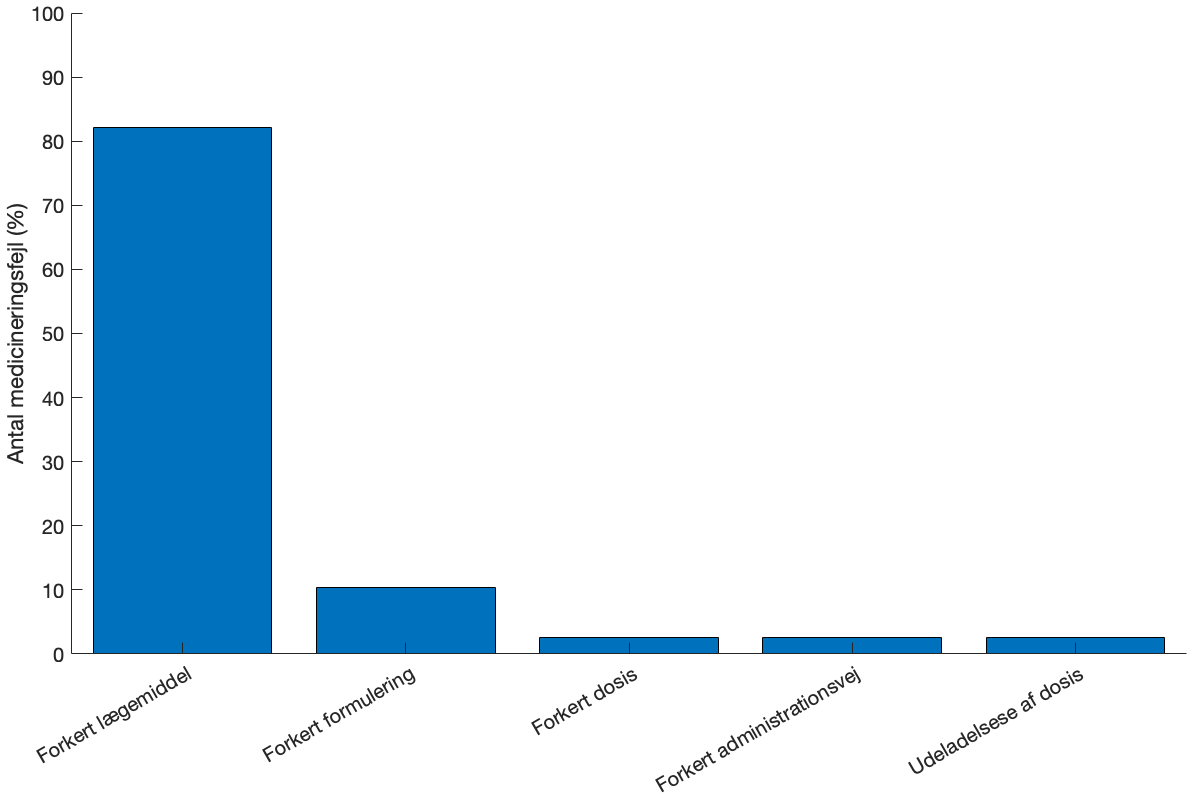
\includegraphics[width=0.95\textwidth]{billeder/GenSubb.png} 
	\caption{Medicineringsfejl ved generisk substitution angivet i procent (n=100)~\citep{Hakonsen2010}.}
	\label{fig:GeneriskSubstitution}  
\end{figure}
\vspace{-0.5cm}

Det fremgår af Figur \ref{fig:GeneriskSubstitution} at størstedelen af fejlmedicinering ved generisk substitution skyldes forkert lægemiddel, hvoraf en mindre del skyldes formulering og i sjældnere tilfælde dosis, administrationsvej og udeladelse af dosis. Forkert lægemiddel sker ved dispensering eller administration af et andet lægemiddel end det forskrevne. Formulering er lægemidlet fysiske form som f.eks. tabellet, dosis er mængden af lægemidlet og administrationsvej er, hvordan indgiften af et lægemiddel indtages. Årsagerne til medicineringsfejl blev rapporteret af 42 sygeplejersker~\citep{Hakonsen2010}, og resultaterne heraf fremgår af Figur \ref{fig:GeneriskSubstitution1}.

\begin{figure}[H]\centering	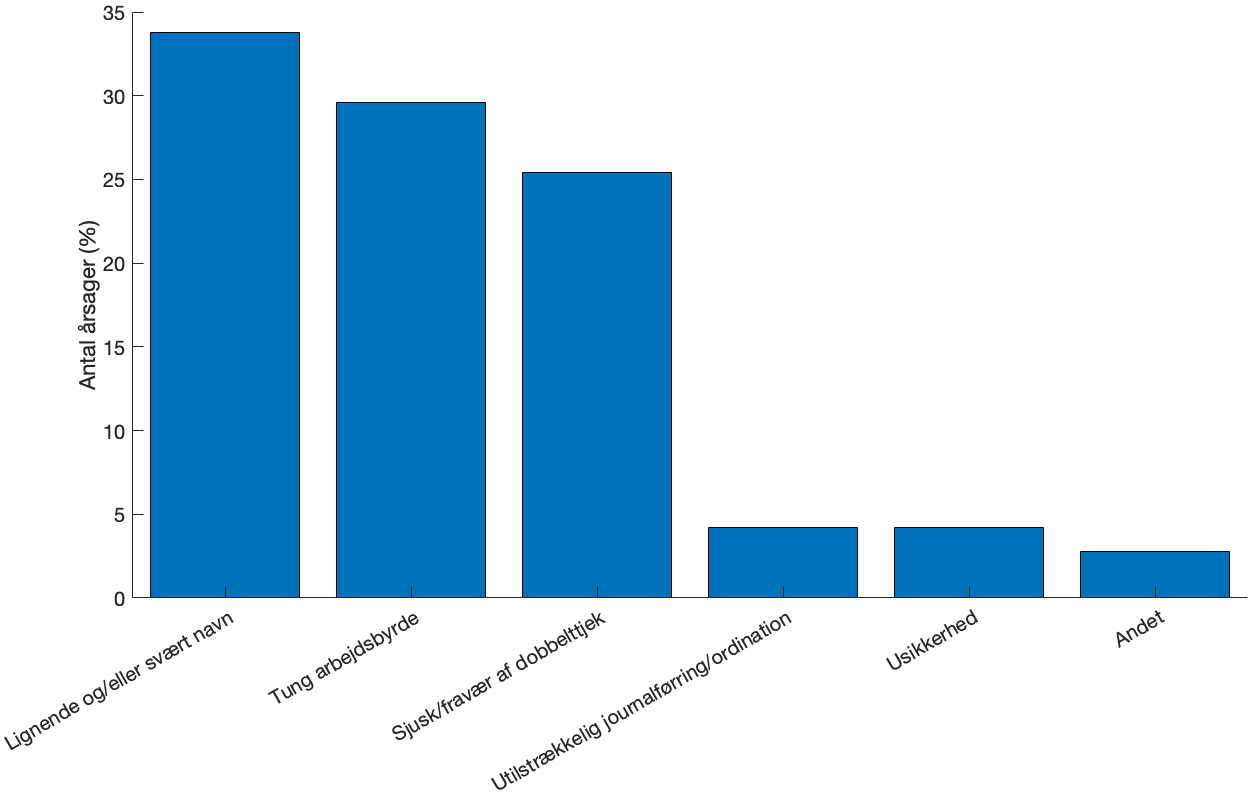
\includegraphics[width=0.95\textwidth]{billeder/GenSubbb.png} 
	\caption{Årsager til medicieringsfejl ved generisk substitution angivet i procent(n=42)~\citep{Hakonsen2010}.}	\label{fig:GeneriskSubstitution1}  
\end{figure}

Det fremgår af Figur \ref{fig:GeneriskSubstitution1} at størstedelen af årsagerne til medicineringsfejl ved generisk substitution skyldes lignende og/eller vanskeligt lægemiddelnavn, kraftig arbejdsbyrde og sløvhed eller fravær af dobbelttjek. En mindre del skyldes utilstrækkeligt journalførring og/eller ordination, usikkerhed eller andet. 

I flere lande opstår forkert lægemiddel ofte i forbindelse med forvirring ved forveksling af navn~\citep{DanskSelskabforPatientsikkerhed2009}, hvilket afspejles i det norske studie. Forveksling af lægemiddelnavne har i sjældnere tilfælde haft konsekvenser som har medført forlænget indlæggelse, forværret sygdom eller dødsfald~\citep{DanskSelskabforPatientsikkerhed2009}. Forveksling af navn kan for eksempel forekomme ved panodil, som er et smertestillende lægemiddel, og plendil, som anvendes til behandling af forhøjet blodtryk~\citep{DanskSelskabforPatientsikkerhed2009}. Derudover kan forskellige suffiks eller præfiks skabe forvirring og give anledning til fejl i dispensering, såsom Efexor kontra Efexor Depot~\citep{DanskSelskabforPatientsikkerhed2009}. Lignede navne, så kaldte look-a-like, såsom dopamin og dobutamin, kan prædisponeres til medicineringsfejl og ligeledes medføre patientsikkerhedsmæssige konsekvenser~\citep{Wittich2014}. Samtidig kan brugen af forkortelser i ordination give anledning til øget risiko for fejlmedicinering~\citep{Wittich2014}.

Nogle af sygeplejerskerne i det norske studie mente at forvirringen over at finde den korrekte substitution kunne lede til at doseringen og formulationen var skyld i medicineringsfejl~\citep{Hakonsen2010}, hvilket kan skyldes at lægemidlets leverandør skiftes, hvormed der foretages substitution og egenskaber ved lægemidlet kan være ændret~\citep{Wittich2014}.

Medicinering var den hyppigste årsag til rapportering af utilsigtede hændelser i Danmark i år 2013~\citep{Patientombuddet2013}. Antallet af rapporteringer i Region Nordjylland er steget med over 36~\% fra år 2012 til 2014~\citep{Jensen2014}. Ud af 824 rapporterede utilsigtede hændelser i år 2014 skyldes 97\% medicinering, 86\% administration af medicin og 41\% disponering~\citep{Jensen2014}, hvor mere end én rapporteret utilsigtede hændelser skyldes én eller flere grunde. Størstedelen af fejl forekommer i forbindelse med ordination og administration, hvoraf en mindre andel sker ved transskribering og dispensering~\citep{Agrawal2009, Anderson2002}. Gentagne årsager i disse studier var forkert dosis og lægemiddel samt udeladelse af ordination, dispensering og administration~\citep{Barker2002,Sundhedsstyrelsen2005,Lisby2005, Tully2009}.

\section{Risikovurderingen af lægemiddelskift} \label{sec:ImpLaeg}
%\textit{Hvorfor foretages en risikovurdering og hvordan foregår denne?} \\
For at forebygge fejlmedicinering og forbedre patientsikkerheden ved lægemiddelskift formidler Sygehusapoteket Region Nordjylland (SRN) information om lægemiddelskift til de enkelte hospitalsafdelinger i regionen med henblik på at opnå en effektiv implementering. Hospitalsafdelingerne informeres om lægemiddelskift via Lægemiddel Nyt, som fremgår af Appendiks \ref{App:LaegemiddelNyt}. Lægemiddel Nyt indeholder oplysninger om lægemiddelskift, der sker på Regions Nordjyllands rekommendationsliste, der er bestemt af Lægemiddelkomitéen~\citep{RegionNordjylland2018}, og hospitalsafsnittenes standardsortimenter. Lægemiddelskift, der er beskrevet af Lægemiddel Nyt, indeholder oplysninger om ændringer i lægemidlets navn, pakningsstørrelse, styrke, opbevaringsbetingelser samt analog substitution. Udover dette er der for særlige lægemidler beskrevet yderligere information, hvilket fremgår af Appendiks \ref{App:LaegemiddelNyt}, hvilket kan være lægemidler, hvor der er ændringer i styrke, dispenseringsform eller udseende.

Lægemiddel Nyt udarbejdes på baggrund af skiftelister, som beskrives af Appendiks \ref{App:Skiftelister}, der indeholder oplysninger som ATC-kode, lægemidlets navn, dispenseringsform, styrke og pakningsstørrelse fra forgående år og året for skiftet. Skiftelisterne anvendes til at undersøge om, der er foretaget ændringer i lægemidlets egenskaber fra foregående år til året for skiftet. Dette markeres manuelt af en medarbejder fra SRN i skiftelisten. Udover dette vurderes kompleksiteten af lægemiddelskiftet af ATC-ansvarlige medarbejder fra SRN ud fra ændringer angivet i skiftelisten og en skabelon til implementering af lægemiddelskift, som fremgår af Appendiks \ref{App:Skabelon}. Ud fra skabelonen tages der stilling til tidspunktet for skiftet, hvilken betydning skiftet kan have for f.eks. klinikken, hvor mange patienter skiftet berører, antallet af hospitalsafsnit som påvirkes, typen af skift f.eks. om det involverer skift af device, samt hvilken metode der skal anvendes til at informerer om skiftet. 

Vurderingen af ændrede egenskaber ved lægemidlet foregår manuelt hvilket gør den tidskrævende og sårbar. Derudover er dele af vurderingen erfaringsbaseret, hvilket gør den personafhængig, da der stilles krav til den enkelte ATC-ansvarlige medarbejders erfaring inden for området. Yderligere er vurderingen baseret på forskellige data fra flere databaser, hvilket foregår manuelt, hvormed nødvendige risikofaktorer som har betydning for skiftet let kan overses og dermed udelades i vurderingen.
Derudover er grundlaget for vurderingen subjektiv, da den afhænger af én ATC-ansvarlige medarbejders viden inden for området og kan derfor være varierende mellem medarbejdere, hvilket gør processen sårbar. En del af vurderingerne er  processorienteret, som f.eks. ændringer i lægemidlets navn, styrke og dispenseringsform, hvilket kan gøres computerbaseret, hvormed denne proces vil være mindre sårbar og personafhængig. Modsat er der dele af vurderingen som er menneskebaseret, hvorved det er nødvendigt at de ATC-ansvarliges viden og erfaring tages med i vurderingen, som f.eks. skiftetidspunkt og skiftets betydning.  

\section{Informationssystemer til forebyggelse og risikovurdering}
%\textit{Hvilke teknologier anvendes til at forebygge medicineringsfejl og risikovurdering? Hvordan kan denne viden anvendes til min problemstilling?} \\



*** OMSTRUKTURER DETTE AFSNIT - SIG DET VIGTIGSTE FØRST - KOM MED EKSEMPLER SOM RELATERE SIG TIL PROJEKTET, SÅ DET IKKE BLIVER FOR GENERELT ***

Ingen videnskabelig litteratur har undersøgt, hvordan informationssystemer kan anvendes til vurderingen af lægemiddelskift inden implementering i klinikken. Den nuværende proces er menneskebaseret og foregår manuel, hvilket gør den sårbar, subjektiv og personafhængig, som beskrevet i Afsnit \ref{sec:ImpLaeg}. Informationssystemer er, modsat den menneskelige evne, i stand til at organisere og identificere sammenhænge mellem informationer fra en større mængde af data~\citep{Agrawal2009}, hvormed den nuværende proces for vurdering af lægemiddelskift kan gøres mere ensartet og vægte flere risikofaktorer, hvilket vil understøtte beslutningsgrundlaget og samtidig gøre processen mindre personafhængig. Derudover kan dele af vurderingen som er procesorienteret blive automatiseret, hvilket gør processen mindre sårbar. 

Flere studier har påvist at informationssystemer er anvendelig i klinikken til forebyggelsen af fejlmedicinering~\citep{Agrawal2009, Kaushal2002, Stenner2010, Fischer2008, Simpson2008, Bates2000a}. Computerbaseret ordineringssystemer anvendes til at strukturere ordre, gøre disse letlæselige og fuldkommen samt gøre nødvendige oplysninger tilgængelige for klinikeren~\citep{Agrawal2009,Bates2000a}. I en kombination med beslutningsstøtte system, som f.eks. interaktion mellem lægemidler og automatisk beregning af styrke ved ændring i denne~\citep{Agrawal2009}, har computerbaseret ordineringssystemer påvist at være effektiv i forbedring af patientsikkerheden~\citep{Agrawal2009, Bates2000a}. Til dispensering anvendes forskellige teknologier som robotter og automatiserede skabe, som anvender stregkoder til at genkende medicin, hvilket medvirker til at reducere antallet af fejl relateret til emballage og dispensering.~\citep{Agrawal2009}.




%Andre studier anvender statistik eller deterministisk metode til risikovurdering \citep{Geissert2018, Boyko1990, Rawshani2018}. Da data er begrænset er det ikke muligt, at målrette problemet og anvende statistisk til at finde sammenhænge mellem dataelementer ved at vægte disse~\citep{Campbell2008,Bruce2007}, hvorfor en deterministisk metode, som opstiller kriterier for dataelementerne ud fra sammenhænge mellem disse kan anvendes~\citep{Campbell2008}. Regelbaseret systemer er deterministiske, og er helt eller delvist bestemt af en ekspert til at repræsentere og automatisere ekspertens viden inden for et begrænset område~\citep{Crina2008}. Da baggrunden for den eksisterende viden inden for området og processerne for vurderingen er kendte kan et regelbaseret system anvendes til risikovurdering.



%Flere studier har påvist at informationssystemer er anvendelig i klinikken til forebyggelsen af fejlmedicinering~\citep{Agrawal2009, Kaushal2002, Stenner2010, Fischer2008, Simpson2008, Bates2000a}. Computerbaseret ordineringssystemer anvendes til at strukturere ordre, gøre disse letlæselige og fuldkommen samt gøre nødvendige oplysninger tilgængelige for klinikeren~\citep{Agrawal2009,Bates2000a}. I en kombination med beslutningsstøtte system, som f.eks. interaktion mellem lægemidler og automatisk beregning af styrke ved ændring i denne~\citep{Agrawal2009}, har computerbaseret ordineringssystemer påvist at være effektiv i forbedring af patientsikkerheden~\citep{Agrawal2009, Bates2000a}. Til dispensering anvendes forskellige teknologier som robotter og automatiserede skabe, som anvender stregkoder til at genkende medicin, hvilket medvirker til at reducere antallet af fejl relateret til emballage og dispensering.~\citep{Agrawal2009}

%Fælles for de ovenstående informationssystemer er, at de anvendes i klinikken, når lægemiddelskiftet er implementeret. Ingen videnskabelig litteratur har undersøgt, om informationssystemer kan anvendes til at opnå en effektiv implementering af lægemiddelskift i klinikken og derved gøre den nuværende vurdering mindre personafhængig og sårbar.Da informationssystemer, modsat den menneskelige evne, er i stand til at organisere og identificere sammenhænge mellem informationer fra en større mængde af data~\citep{Agrawal2009}, vil dette medvirke til at processen bliver mere ensartet, da flere risikofaktorer kan vægtes i vurderingen af lægemiddelskift, hvilket understøtte beslutningsgrundlaget, og gøre processen mindre personafhængig. Herved kan flere risikofaktorer vægtes i vurderingen af lægemiddelskift, hvilket ligeledes vil understøtte beslutningsgrundlaget. Derudover vil vurdering blive automatiseret, hvilket vil gøre processen mindre sårbar. 

%Andre studier anvender statistik eller deterministisk metode til risikovurdering \citep{Geissert2018, Boyko1990, Rawshani2018}. Da data er begrænset er det ikke muligt, at målrette problemet og anvende statistisk til at finde sammenhænge mellem dataelementer ved at vægte disse~\citep{Campbell2008,Bruce2007}, hvorfor en deterministisk metode, som opstiller kriterier for dataelementerne ud fra sammenhænge mellem disse kan anvendes~\citep{Campbell2008}. Regelbaseret systemer er deterministiske, og er helt eller delvist bestemt af en ekspert til at repræsentere og automatisere ekspertens viden inden for et begrænset område~\citep{Crina2008}. Da baggrunden for den eksisterende viden inden for området og processerne for vurderingen er kendte kan et regelbaseret system anvendes til risikovurdering.

\section{Opsummering}
Lægemiddelskift sker for at sænke udgifterne til sygehusmedicin, hvilket medfører substitution af lægemidler ~\citep{Ess2003, Johnston2011}. Substitution af lægemidler og hvor godt disse implementeres i klinikken har betydning for forebyggelsen af medicineringsfejl og derved forbedring af patientsikkerheden, jævnfør Afsnit \ref{sec:ProblemLaeg}. Den nuværende vurdering af kompleksiteten af lægemiddelskift inden implementering i klinikken foregår manuelt og er derfor sårbar, som beskrevet i Afsnit \ref{sec:ImpLaeg}. Ligeledes er den erfaringsbaseret og subjektiv, hvilket gør processen personafhængig.

Studier har påvist at informationssystemer kan anvendes til at reducere antallet af medicineringsfejl i klinikken~\citep{Agrawal2009, Stenner2010, Fischer2008, Simpson2008}, men ingen videnskabelig litteratur har undersøgt informationssystemer til at vurdere lægemiddelskift inden implementering i klinikken. Da processen og erfaringer er kendte for vurdering af lægemiddelskift kan regelbaseret systemer anvendes til at repræsentere og automatisere denne viden. Ud fra en deterministisk metode er det muligt at sammenligne data fra flere databaser, hvormed processen kan blive mindre personafhængig og sårbar.

\section{Problemformulering}
\textit{Hvilken anvendelighed har et regelbaseret system til risikovurdering af lægemiddelskift med henblik på at forbedre den nuværende vurdering af lægemiddelskift?}

%\textit{risikovurdering af lægemiddelskift foretaget af ATC-ansvarlige medarbejdere på SRN? \textcolor{blue}{med henblik på at effektivisere implementering af kommende lægemiddelskift ved udarbejdelsen af LægemiddelNyt?} }



